\section{Resultados}
\subsection{Experimentacion con Imagenes Reducidas}
\subsubsection{Metodo 0: Utilizando $A^tA$}

\underline{\textbf{Mediciones de TK \textcolor{red}{Explicar que es esto}}}

\begin{figure}[H]
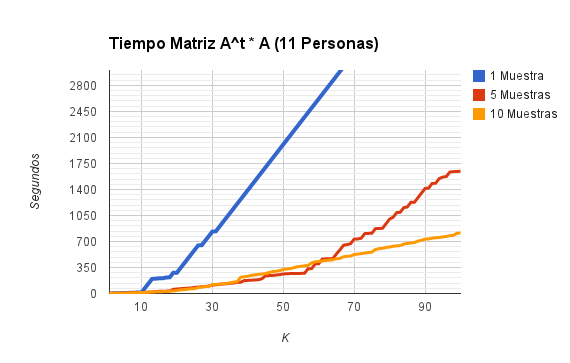
\includegraphics[width=1\textwidth]{img/image1.png}
     \caption{Tiempos Matrix $A^tA$ con 11 personas variando K}
     \label{fig:figura1}
\end{figure}

\begin{figure}[H]
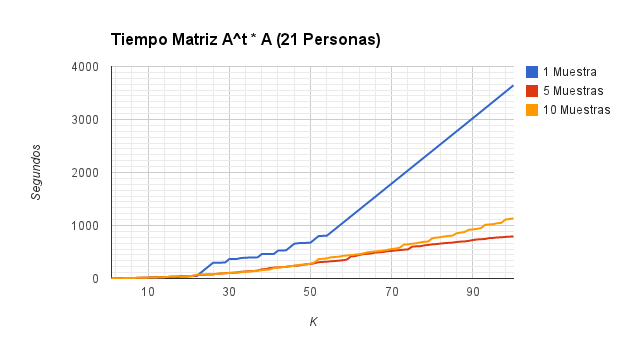
\includegraphics[width=1\textwidth]{img/image2.png}
     \caption{Tiempos Matrix $A^tA$ con 21 personas variando K}
     \label{fig:figura1}
\end{figure}

\begin{figure}[H]
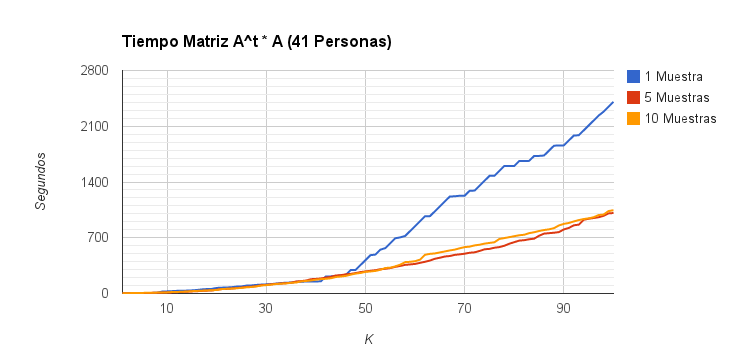
\includegraphics[width=1\textwidth]{img/image3.png}
     \caption{Tiempos Matrix $A^tA$ con 41 personas variando K}
     \label{fig:figura1}
\end{figure}


\underline{\textbf{Mediciones de Ttodos \textcolor{red}{Explicar que es esto}}}

\begin{figure}[H]
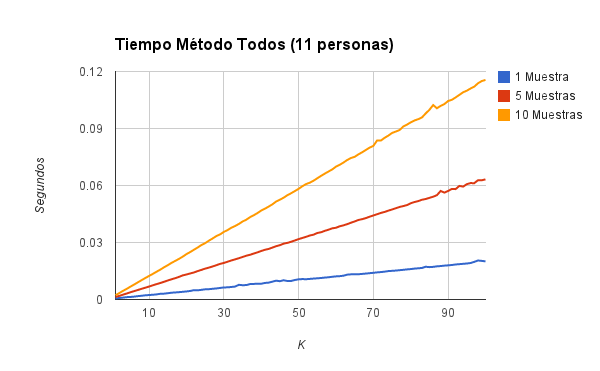
\includegraphics[width=1\textwidth]{img/image4.png}
     \caption{Tiempos Todos \textcolor{red}{??} Matrix $A^tA$ con 11 personas variando K}
     \label{fig:figura1}
\end{figure}

\begin{figure}[H]
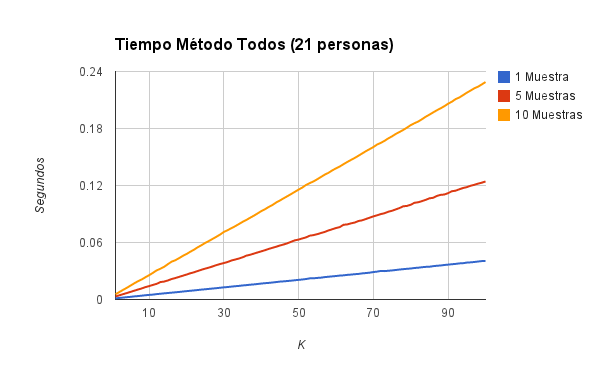
\includegraphics[width=1\textwidth]{img/image5.png}
     \caption{Tiempos Todos \textcolor{red}{??} Matrix $A^tA$ con 21 personas variando K}
     \label{fig:figura1}
\end{figure}

\begin{figure}[H]
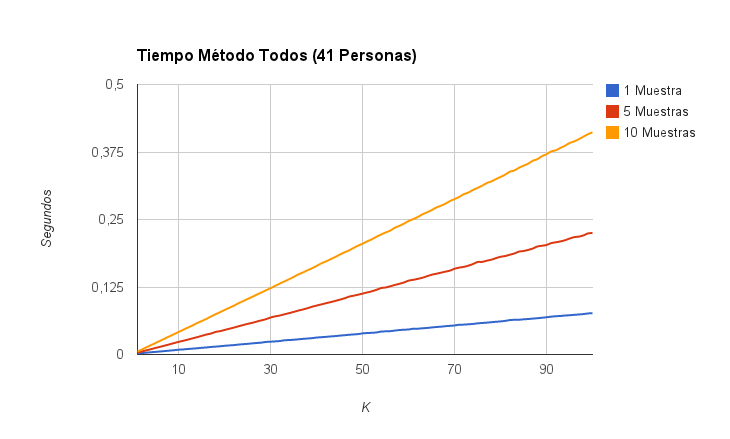
\includegraphics[width=1\textwidth]{img/image6.png}
     \caption{Tiempos Todos \textcolor{red}{??} Matrix $A^tA$ con 41 personas variando K}
     \label{fig:figura1}
\end{figure}


\underline{\textbf{Mediciones de Tcentro \textcolor{red}{Explicar que es esto}}}

\begin{figure}[H]
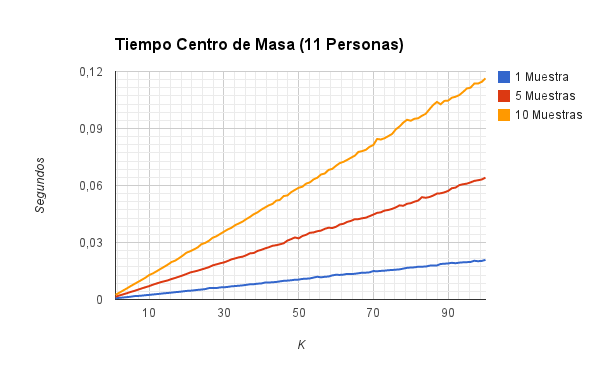
\includegraphics[width=1\textwidth]{img/image7.png}
     \caption{Tiempos Centro \textcolor{red}{??} Matrix $A^tA$ con 11 personas variando K}
     \label{fig:figura1}
\end{figure}

\begin{figure}[H]
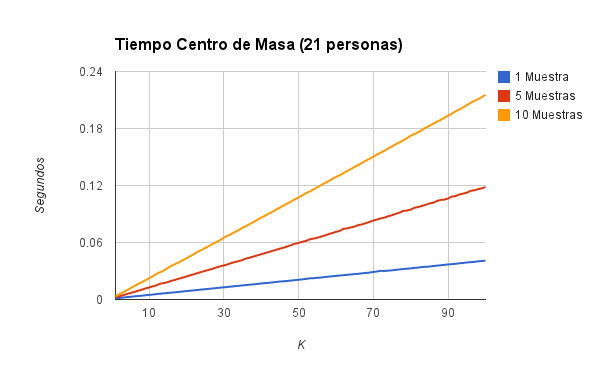
\includegraphics[width=1\textwidth]{img/image8.png}
     \caption{Tiempos Centro \textcolor{red}{??} Matrix $A^tA$ con 21 personas variando K}
     \label{fig:figura1}
\end{figure}

\begin{figure}[H]
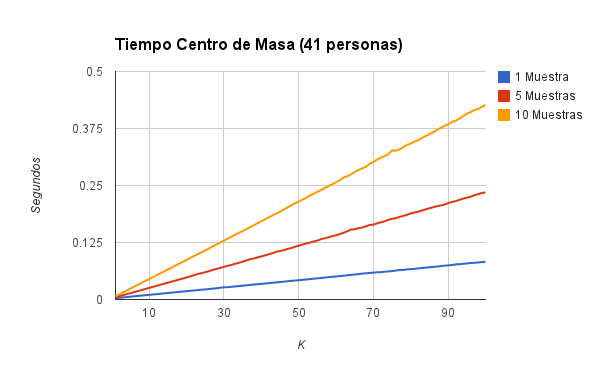
\includegraphics[width=1\textwidth]{img/image9.png}
     \caption{Tiempos Centro \textcolor{red}{??} Matrix $A^tA$ con 41 personas variando K}
     \label{fig:figura1}
\end{figure}



\underline{\textbf{Mediciones de HitsTodos \textcolor{red}{Explicar que es esto}}}

\begin{figure}[H]
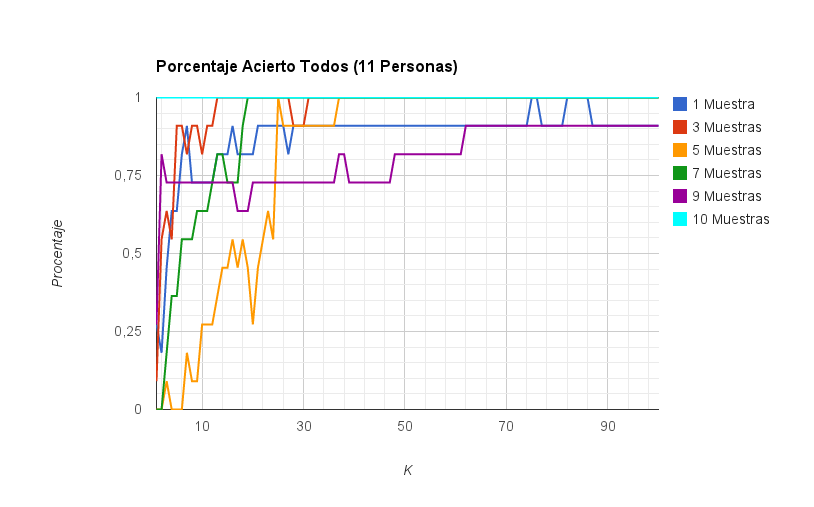
\includegraphics[width=1\textwidth]{img/image10.png}
     \caption{Tiempos HitTodos \textcolor{red}{??} Matrix $A^tA$ con 11 personas variando K}
     \label{fig:figura1}
\end{figure}

\begin{figure}[H]
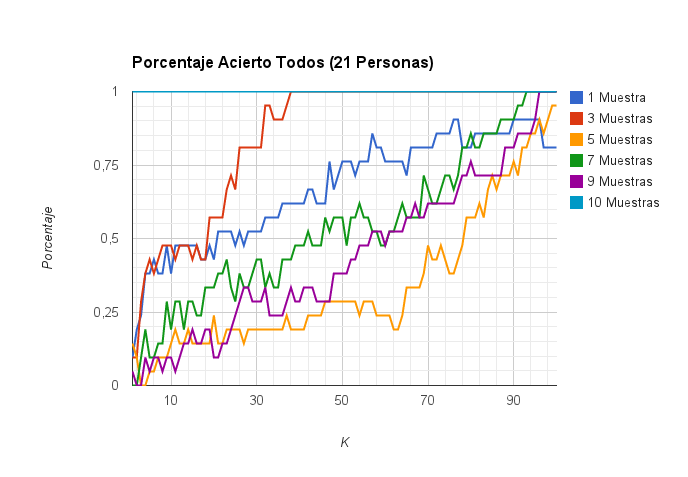
\includegraphics[width=1\textwidth]{img/image11.png}
     \caption{Tiempos HitTodos \textcolor{red}{??} Matrix $A^tA$ con 21 personas variando K}
     \label{fig:figura1}
\end{figure}

\begin{figure}[H]
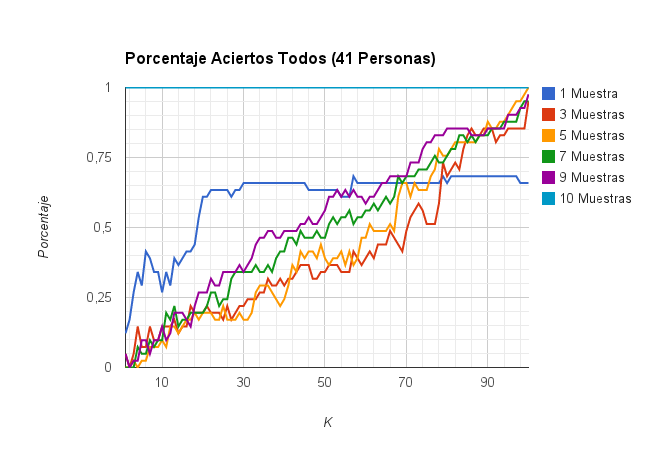
\includegraphics[width=1\textwidth]{img/image12.png}
     \caption{Tiempos HitTodos \textcolor{red}{??} Matrix $A^tA$ con 41 personas variando K}
     \label{fig:figura1}
\end{figure}





\underline{\textbf{Mediciones de HitsCentro \textcolor{red}{Explicar que es esto}}}

\begin{figure}[H]
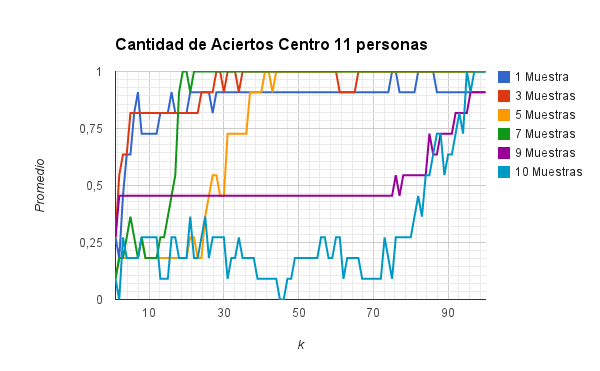
\includegraphics[width=1\textwidth]{img/image13.png}
     \caption{Tiempos HitsCentro \textcolor{red}{??} Matrix $A^tA$ con 11 personas variando K}
     \label{fig:figura1}
\end{figure}

\begin{figure}[H]
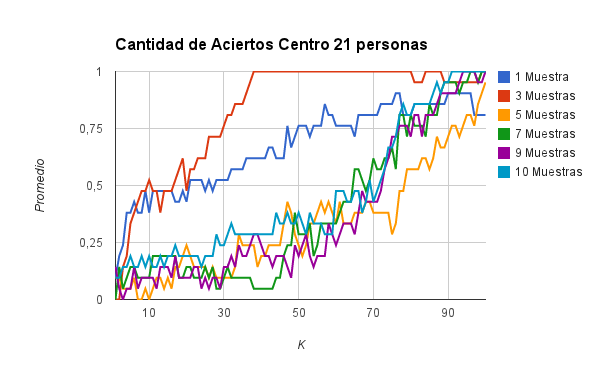
\includegraphics[width=1\textwidth]{img/image14.png}
     \caption{Tiempos HitsCentro \textcolor{red}{??} Matrix $A^tA$ con 21 personas variando K}
     \label{fig:figura1}
\end{figure}

\begin{figure}[H]
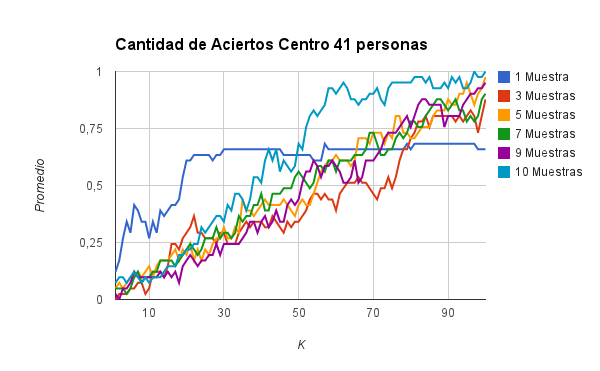
\includegraphics[width=1\textwidth]{img/image15.png}
     \caption{Tiempos HitsCentro \textcolor{red}{??} Matrix $A^tA$ con 41 personas variando K}
     \label{fig:figura1}
\end{figure}

\underline{\textbf{Conclusiones:}}

\textcolor{red}{EXPLICAR}


\subsubsection{Metodo 1: Utilizando $AA^t$}

\underline{\textbf{Mediciones de TK \textcolor{red}{Explicar que es esto}}}

\begin{figure}[H]
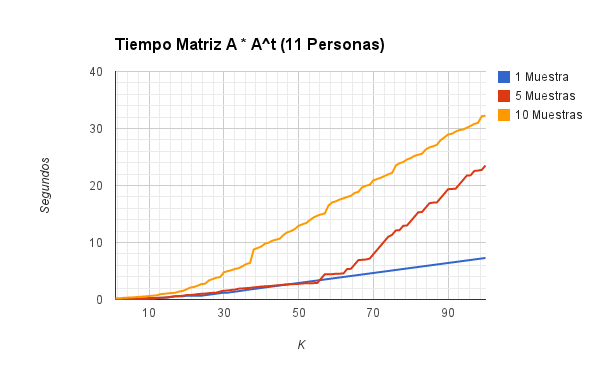
\includegraphics[width=1\textwidth]{img/imagea.png}
     \caption{Tiempos Matrix $A^tA$ con 11 personas variando K}
     \label{fig:figura1}
\end{figure}

\begin{figure}[H]
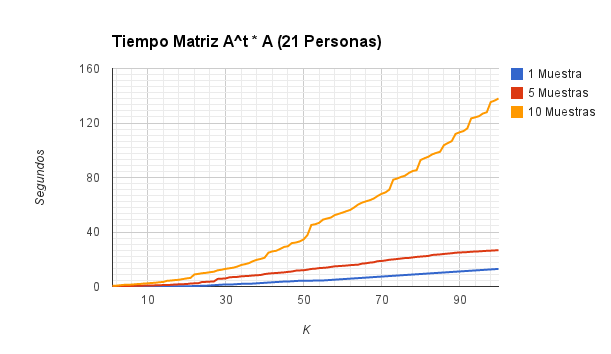
\includegraphics[width=1\textwidth]{img/imageb.png}
     \caption{Tiempos Matrix $A^tA$ con 21 personas variando K}
     \label{fig:figura1}
\end{figure}

\begin{figure}[H]
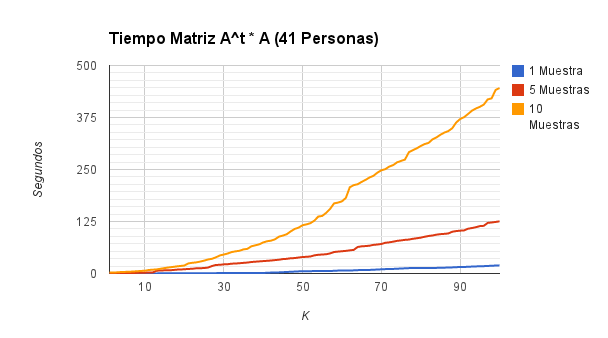
\includegraphics[width=1\textwidth]{img/imagec.png}
     \caption{Tiempos Matrix $A^tA$ con 41 personas variando K}
     \label{fig:figura1}
\end{figure}


\underline{\textbf{Mediciones de Ttodos \textcolor{red}{Explicar que es esto}}}

\begin{figure}[H]
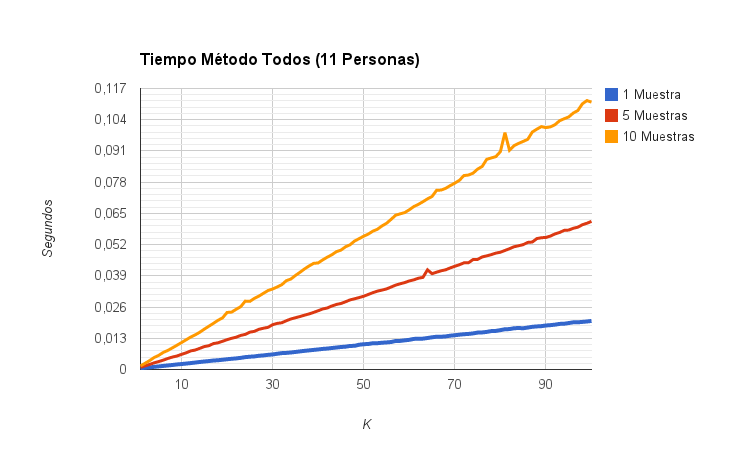
\includegraphics[width=1\textwidth]{img/imaged.png}
     \caption{Tiempos Todos \textcolor{red}{??} Matrix $A^tA$ con 11 personas variando K}
     \label{fig:figura1}
\end{figure}

\begin{figure}[H]
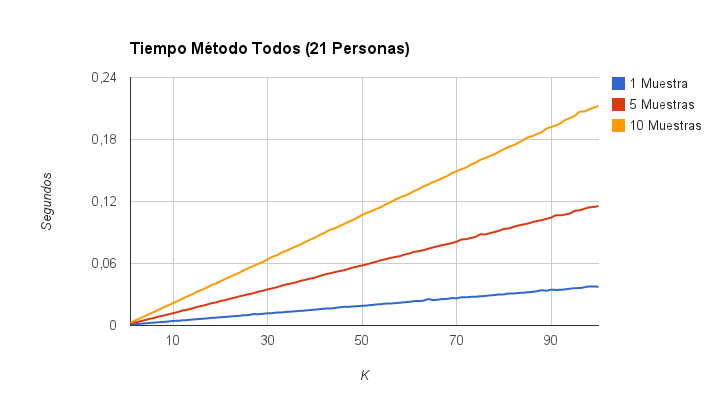
\includegraphics[width=1\textwidth]{img/imagee.png}
     \caption{Tiempos Todos \textcolor{red}{??} Matrix $A^tA$ con 21 personas variando K}
     \label{fig:figura1}
\end{figure}

\begin{figure}[H]
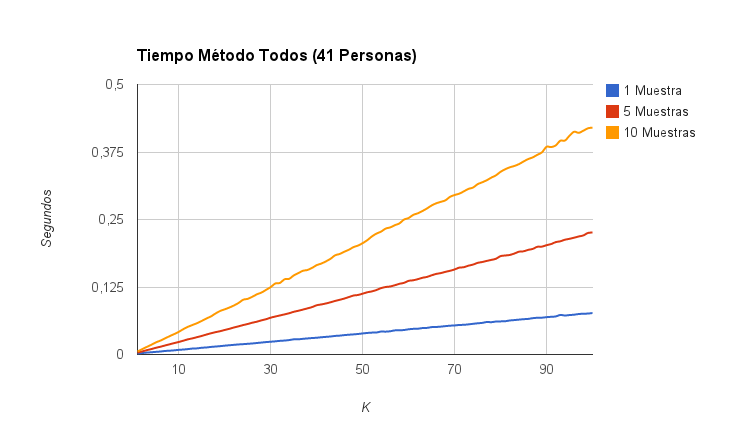
\includegraphics[width=1\textwidth]{img/imagef.png}
     \caption{Tiempos Todos \textcolor{red}{??} Matrix $A^tA$ con 41 personas variando K}
     \label{fig:figura1}
\end{figure}

\underline{\textbf{Mediciones de Tcentro \textcolor{red}{Explicar que es esto}}}

\begin{figure}[H]
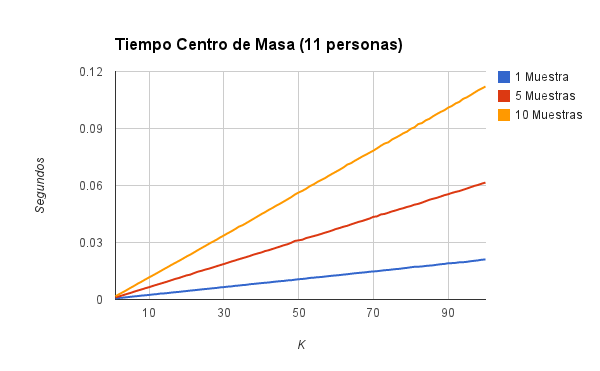
\includegraphics[width=1\textwidth]{img/imageg.png}
     \caption{Tiempos Centro \textcolor{red}{??} Matrix $A^tA$ con 11 personas variando K}
     \label{fig:figura1}
\end{figure}

\begin{figure}[H]
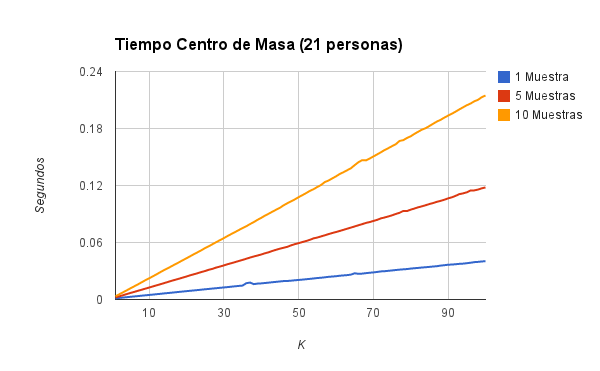
\includegraphics[width=1\textwidth]{img/imageh.png}
     \caption{Tiempos Centro \textcolor{red}{??} Matrix $A^tA$ con 21 personas variando K}
     \label{fig:figura1}
\end{figure}

\begin{figure}[H]
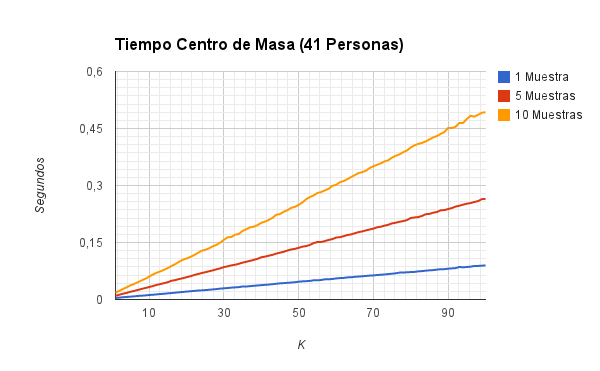
\includegraphics[width=1\textwidth]{img/imagei.png}
     \caption{Tiempos Centro \textcolor{red}{??} Matrix $A^tA$ con 41 personas variando K}
     \label{fig:figura1}
\end{figure}


\underline{\textbf{Mediciones de HitsTodos \textcolor{red}{Explicar que es esto}}}

\begin{figure}[H]
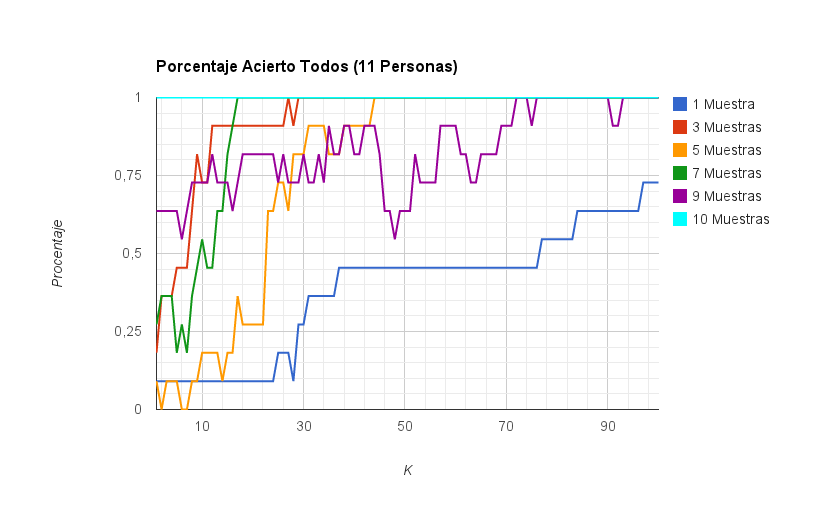
\includegraphics[width=1\textwidth]{img/imagej.png}
     \caption{Tiempos HitTodos \textcolor{red}{??} Matrix $A^tA$ con 11 personas variando K}
     \label{fig:figura1}
\end{figure}

\begin{figure}[H]
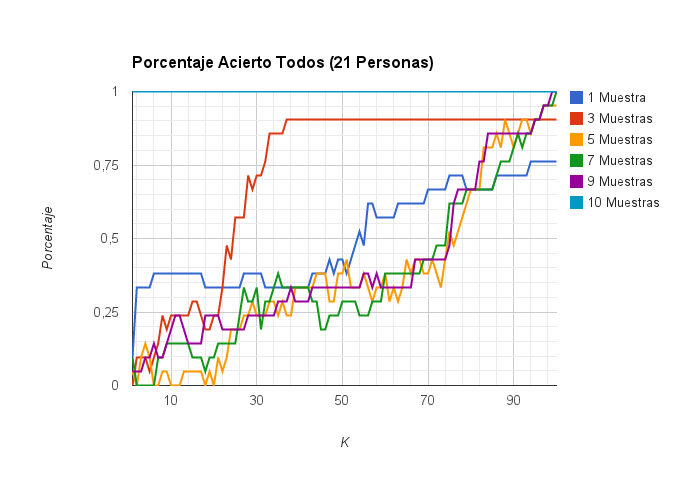
\includegraphics[width=1\textwidth]{img/imagek.png}
     \caption{Tiempos HitTodos \textcolor{red}{??} Matrix $A^tA$ con 21 personas variando K}
     \label{fig:figura1}
\end{figure}

\begin{figure}[H]
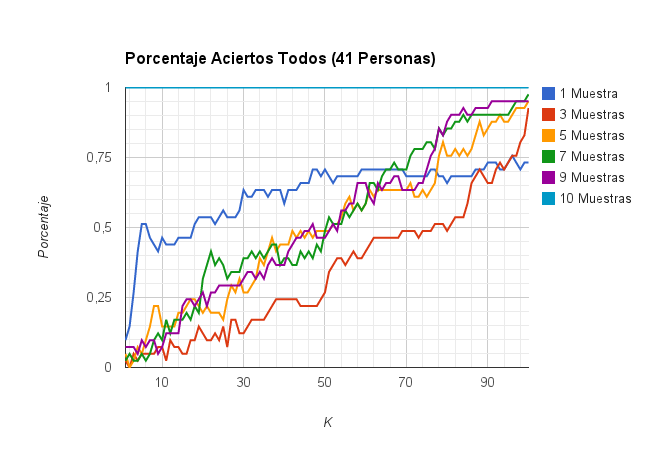
\includegraphics[width=1\textwidth]{img/imagel.png}
     \caption{Tiempos HitTodos \textcolor{red}{??} Matrix $A^tA$ con 41 personas variando K}
     \label{fig:figura1}
\end{figure}

\underline{\textbf{Mediciones de HitsCentro \textcolor{red}{Explicar que es esto}}}

\begin{figure}[H]
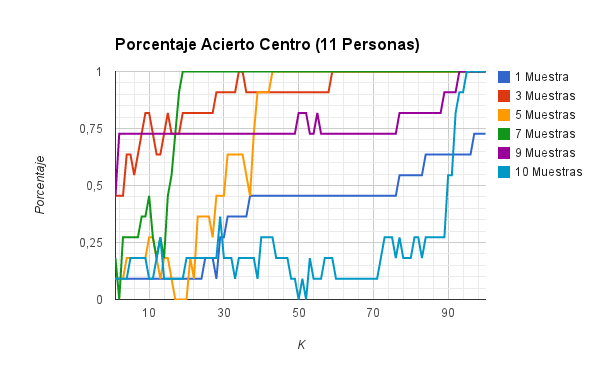
\includegraphics[width=1\textwidth]{img/imagem.png}
     \caption{Tiempos HitsCentro \textcolor{red}{??} Matrix $A^tA$ con 11 personas variando K}
     \label{fig:figura1}
\end{figure}

\begin{figure}[H]
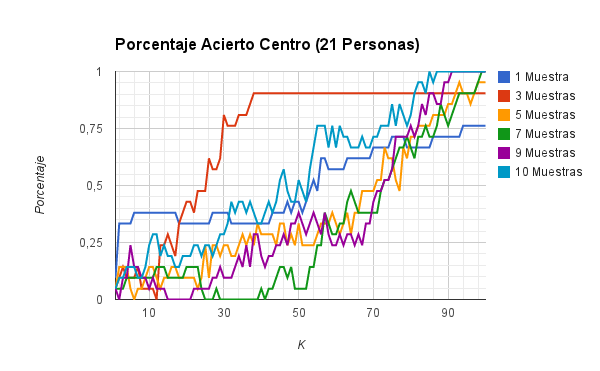
\includegraphics[width=1\textwidth]{img/imagen.png}
     \caption{Tiempos HitsCentro \textcolor{red}{??} Matrix $A^tA$ con 21 personas variando K}
     \label{fig:figura1}
\end{figure}

\begin{figure}[H]
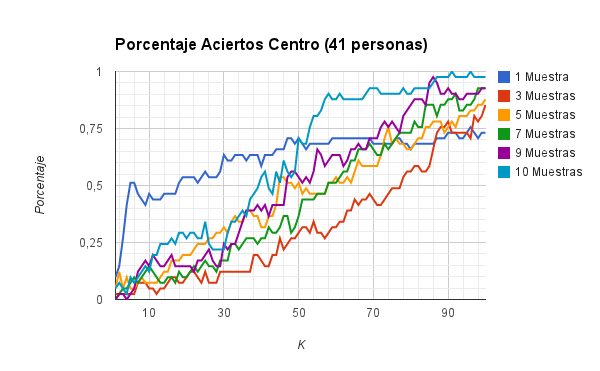
\includegraphics[width=1\textwidth]{img/imager.png}
     \caption{Tiempos HitsCentro \textcolor{red}{??} Matrix $A^tA$ con 41 personas variando K}
     \label{fig:figura1}
\end{figure}

\underline{\textbf{Conclusiones:}}

\textcolor{red}{EXPLICAR}

\subsection{Experimentacion con Imagenes Full}

\subsubsection{Metodo 0: Utilizando $A^tA$}

\underline{\textbf{Mediciones de TK \textcolor{red}{Explicar que es esto}}}

\underline{\textbf{Mediciones de Ttodos \textcolor{red}{Explicar que es esto}}}

\underline{\textbf{Mediciones de Tcentro \textcolor{red}{Explicar que es esto}}}

\underline{\textbf{Mediciones de HitsTodos \textcolor{red}{Explicar que es esto}}}

\underline{\textbf{Mediciones de HitsCentro \textcolor{red}{Explicar que es esto}}}

\underline{\textbf{Conclusiones:}}

\textcolor{red}{EXPLICAR}

\subsubsection{Metodo 1: Utilizando $AA^t$}

\underline{\textbf{Mediciones de TK \textcolor{red}{Explicar que es esto}}}

\underline{\textbf{Mediciones de Ttodos \textcolor{red}{Explicar que es esto}}}

\underline{\textbf{Mediciones de Tcentro \textcolor{red}{Explicar que es esto}}}

\underline{\textbf{Mediciones de HitsTodos \textcolor{red}{Explicar que es esto}}}

\underline{\textbf{Mediciones de HitsCentro \textcolor{red}{Explicar que es esto}}}

\underline{\textbf{Conclusiones:}}

\textcolor{red}{EXPLICAR}
